\chapter{Software tester}
\section{G\'{e}n\'{e}ralit\'{e}s sur le test}
Interview avec Fabien




\section{Le test \`{a} SAP}

!!!!!!!!!!!Pr\'{e}senter l'architecture de test et les diff\'{e}rents process!!!!!!!!!!!!!\\

L'\'{e}quipe Tranverse est particuli\`{e}rement foculis\'{e}e d'une part, sur le test coverage\index{Test coverage}, les tests de r\'{e}gression, les tests de performance; et d'autre part sur le principe \textquote{un bug un test}. Ce principe consiste, comme son nom l'indique, que chacun des bugs fix\'{e}s par un d\'{e}veloppeur soit syst\'{e}matiquement test\'{e} par un ST\index{Software Tester}

SAP utilise un grand nombre d'outils pour g\'{e}rer le code de ses nombreux produits, poss\'{e}dant chacun plusieurs branches, ayant chacune une suite de tests ex\'{e}cut\'{e}e quotidiennement. Globalement les codes, quels qu'ils soient, sont h\'{e}berg\'{e}s sur le gestionnaire de code source Perforce\index{Perforce}. La compilation journali\`{e}re est ex\'{e}cut\'{e}e par Jenkins ou ASTEC, d\'{e}pendamment des \'{e}quipes et des produits, dont les r\'{e}sultats sont automatiquement envoy\'{e}s aux personnes concern\'{e}es (cf. annexe \ref{pdf:automationResults} page \pageref{pdf:automationResults} qui pr\'{e}sente l'un de ces mails automatiques).\\



Les ST\index{Software Tester} sont r\'{e}guli\`{e}rement tenus au fait des tests \`{a} impl\'{e}menter aussi bien par Jira\index{Jira} ou Java Correction WorkBench\index{Java Correction WorkBench} que par liste de distribution de mails (cf. figure \ref{figure:testProcess} page \pageref{figure:testProcess} pour le process complet)\\
\begin{figure}[!h]
  \centering
      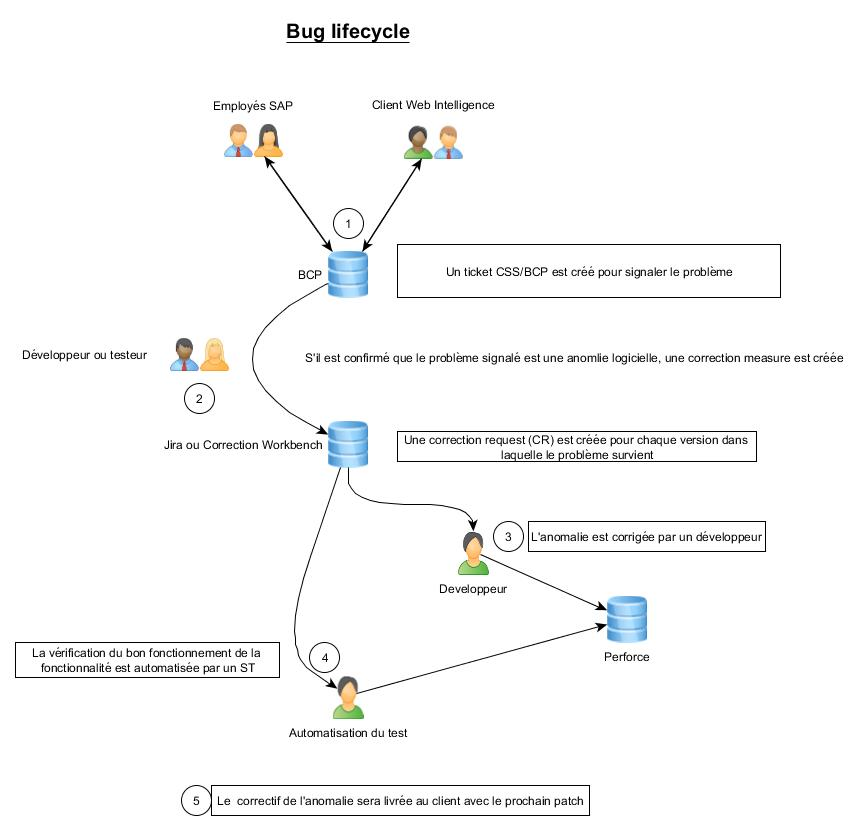
\includegraphics[width=\textwidth]{images/testProcessAtSAP.jpg}
  \caption{Le process de test}
	\label{figure:testProcess}
\end{figure}



\section{Pr\'{e}sentation du produit test\'{e} : WebI}
WebI est un logiciel de BI\index{Business Intelligence} permettant d'acc\'{e}der \`{a} des donn\'{e}es stock\'{e}es en ligne dans un \textquote{univers} (anciennement des fichiers aux extensions .unv, mainteant .unx). L'acc\`{e}s aux donn\'{e}es peut se faire via rich client\index{Rich Client} via applet ou via le client dhtml.


\section{Pr\'{e}paration aux tests}

Mes 1\up{er} jours \`{a} SAP se sont d\'{e}roul\'{e}s de la mani\`{e}re suivante :\\
\begin{itemize}
\item Pr\'{e}sentation \`{a} l'\'{e}quipe et visite des locaux
\item R\'{e}union avec mon tuteur et mon manager pour une description de la mission
\item R\'{e}cup\'{e}ration des diff\'{e}rents droits d'acc\`{e}s aux serveurs
\item Familiarisation avec les outils internes (tickets HR, CSS, IT, ...)
\item Installation des logiciels n\'{e}cessaires au d\'{e}veloppement (IDE, SCM\index{Source Code Management}, \'{e}diteur de texte)
\item Mise en place du framework de test (cr\'{e}ation workspace perforce) \`{a} l'aide de Christophe DOLIMONT
\item Au terme de la 1\up{\`{e}re} semaine, j'ai pu commencer \`{a} utiliser le framework de test en me basant sur les tests d\'{e}j\`{a} existants
\end{itemize}

Une fd

%\glspl{pois} \\
%\glspl{vache} \\
%\glspl{pigeon} \\
% \glspl{TEM}  \\
% \gls{latex}  \\
%\glspl{lvm}




\section{D\'{e}roulement de la 1\up{\`{e}me} mission}

!!!!!cf journal de bord tests!!!!!!!!!!!\\
!!!!! caract\'{e}ristique de base de WebI!!!!!!!!!!!\\
L'objectif principal de cette mission \'{e}tait d'\^{e}tre, \`{a} terme, capable d'impl\'{e}menter seul un test automatique. La difficult\'{e} majeure rencontr\'{e}e au d\'{e}but de cette p\'{e}riode \`{a} \'{e}t\'{e} de comprendre la logique de test du framework\index{Framework} de test. Les points suivants sont importants pour pouvoir utiliser le framework correctement : 
\begin{itemize}
	\item L'int\'{e}gration du test \`{a} la suite de tests 
  \item Quel type de test mettre en place, statique ou dynamique?
	\item Comment initialiser un test, les constructeurs des tests dynamiques peuvent se baser sur un lcmbiar\index{lcmbiar}, un wid\index{wid} ou une queryspec\index{queryspec}
	\item Les tests ne se basant pas sur les m\^{e}mes versions du produits, les JARs\index{JAR} ne sont jamais les m\^{e}mes
	\item Où trouver les fichiers n\'{e}cessaires
\end{itemize}




\subsection{Tests statiques ou dynamiques}

Le test, qu'il soit statique ou dynamique, sera exécuté avec tous les autres dès lors que le nom du test plan est inscrit dans la test suite.\\
La différence fonctionnelle entre ces deux types de tests est que l'un ne fait que comparer deux doc alors que l'autre fait des modifications sans nécessairement le comparer à une référence.\\
La différence horaire est très importante, pour un test statique il n'est pas nécessaire d'implémenter de testcase! Il suffit de générer la référence, de la mettre dans le dossier dédié, compléter le script.xml et la test suite, implémenter le test plan et commit. 

\subsubsection{Tests statiques}
Le test statique

\begin{itemize}
	\item ne fait que comparer un document par rapport \`{a} une r\'{e}f\'{e}rence, aucun testcase\index{Testcase} n'est donc \`{a} impl\'{e}menter
	\item ne demande que très peu de connaissances technique, que ce soit en Java ou sur WebI
\end{itemize}

Lors de l'ex\'{e}cution d'un test statique, un fichier est g\'{e}n\'{e}r\'{e} \`{a} partir d'un wid\index{wid}, son format (txt\_\footnote{type personnalis\'{e} interne \`{a} SAP}, txt ou doc) est pr\'{e}cis\'{e} dans le fichier script.xml.\\
Ensuite, à la fin de l'ex\'{e}cution du test, ce fichier g\'{e}n\'{e}r\'{e} est compar\'{e} avec un fichier de r\'{e}f\'{e}rence (ce fichier de r\'{e}f\'{e}rence \'{e}tant g\'{e}n\'{e}r\'{e} par le ST\index{Software Tester} lors de l'impl\'{e}mentation de son test en mettant l'option savingtxt à true).\\
Si les deux fichier sont identiques le test est correct, sinon il \'{e}choue.\\
Pour l'exécution d'un test statique il ne faut qu'implémenter un testplan qui respecte la structure suivante :

\lstinputlisting[language=java]{scripts/basicStaticTest.java}




\subsubsection{Tests dynamiques}

\`{A} la diff\'{e}rence du test statique, le test dynamique va modifier le document apr\`{e}s ouverture. Ceci permettant de s'assurer que la m\'{e}canique interne de WebI produit l'effet escompt\'{e} sur le document. La comparaison avec un document de r\'{e}f\'{e}rence est bien \'{e}videmment possible.\\
Un testplan respecte l'impl\'{e}mentation suivante :


\lstinputlisting[language=java]{scripts/basicDynamicTestPlan.java}


Et son testcase respecte l'impl\'{e}mentation suivante :

\lstinputlisting[language=java]{scripts/basicDynamicTestCase.java}

\`{A} la lecture du test case on peut observer le constructeur de la super classe, celui-ci prends un certain nombre d'arguments. Il existe 10 constructeurs différents pour la super classe MonoDocTestCase mais 2 sont particulièrement important. L'un permet de baser son test sur un document généré à partir d'une queryspec\index{queryspec}, l'autre sur un document .wid\index{wid}. Par exemple le constructeur se basant sur un wid\index{wid} :\\
\begin{lstlisting}
MonoDocTestCase(MonoDocTestCaseConfigInfo tccInfo, String sDocumentName, String sCategoryType, String sCategory, Boolean useAuroraCtx);
\end{lstlisting}
où
\begin{description}
	\item[tccInfo] \hfill \\
	Objet contenant les informations générales relatives au test case
	\item[sDocumentName] \hfill \\
	Nom du document .wid\index{wid} qui sera chargé lors de la construction de l'objet
	\item[sCategoryType] \hfill \\
	Nom de la catégorie, en général : \textquote{corporate}
	\item[sCategory] \hfill \\
	Path du dossier dans lequel est stocké le .wid\index{wid}. Doit respecter la nomenclature suivante : /auto/\{scriptname\}/wid\index{wid}
	\item[useAuroraCtx] \hfill \\
	Le test en question porte t-il sur aurora?
\end{description}
 Dans tous les cas, lorsque l'objet testcase est instancié, nous pouvons implémenter un code manipulant le document au niveau SDK\index{SDK}; ce qui signifie que l'on ne simule pas un clic sur un bouton mais que l'on appel l'une des méthodes \textquote{derrière} ce bouton, reproduisant ainsi le comportement d'une manipulation au niveau GUI\index{Graphical User Interface}



\subsubsection{Exécution d'un test}


Lors de l'exécution d'un test plusieurs fichiers sont générés en divers endroits, il y a par exemple :
\begin{description}
\item[Des fichiers de log] \hfill \\ sd
\item[La sortie console] \hfill \\
Enregistrée dans \\ \ldots\textbackslash{}Workspace\_Aurora\textbackslash{}rebean\textbackslash{}logs\textbackslash{}\{scriptname\}
\item[Les fichiers générés] \hfill \\
Enregistrés dans \\ \ldots\textbackslash{}Workspace\_Aurora\textbackslash{}rebean\textbackslash{}results\textbackslash{}Your Build Number\textbackslash{}res\textbackslash{}\{ scriptName\}\textbackslash{}CM\_\{cmNumber\}\_\{short text\}\textbackslash{}\\
uniquement si l'enregistrement des ressources est spécifié dans le script.xml\\
Si savingDoc est à True le document de référence est enregistré sur le CMS\index{CMS} dans le dossier Folders/Public Folders/auto/, voir l'illustration \ref{figure:savedReferenceDocPath} page \pageref{figure:savedReferenceDocPath}, et le document généré est enregistré dans My Documents/My Favorites/Personnals Documents, voir l'illustration \ref{figure:savedGeneratedDocPath} page \pageref{figure:savedGeneratedDocPath}
\begin{figure}[!h]
  \centering
      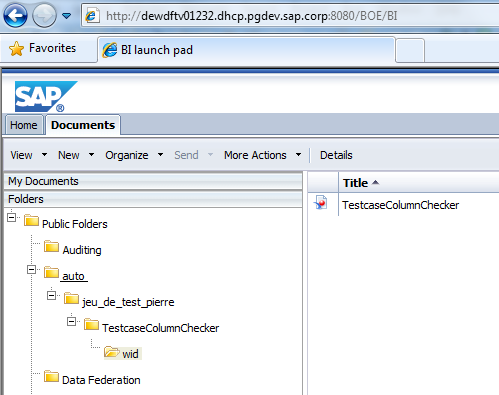
\includegraphics{images/savedReferenceDocPath.png}
  \caption{Capture d'écran de WebI de l'arborescence du document de référence}
	\label{figure:savedReferenceDocPath}
\end{figure}
\begin{figure}[!h]
  \centering
      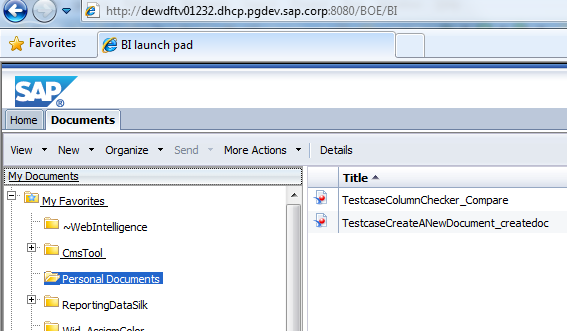
\includegraphics{images/savedGeneratedDocPath.png}
  \caption{Capture d'écran de WebI de l'arborescence du document généré}
	\label{figure:savedGeneratedDocPath}
\end{figure}


\item[Les fichiers de référence] \hfill \\
Les .wid\index{wid} sont enregistrés dans \\ \ldots\textbackslash{}Resources\_AURORA\textbackslash{}storage\textbackslash{}auto\textbackslash{}\{ scriptName\}\textbackslash{}wid\index{wid}\\
et les autres documents de références (txt, html, etc.) sont dans \\ \ldots\textbackslash{}Resources\_AURORA\textbackslash{}storage\textbackslash{}auto\textbackslash{}\{scriptName\}\textbackslash{}CM\_\{cmNumber\}\_\{short text\}\textbackslash{}\\ 
voir une illustration de cette arborescence figure \ref{figure:localSavedReferences} page \pageref{figure:localSavedReferences}
\begin{figure}[!h]
  \centering
      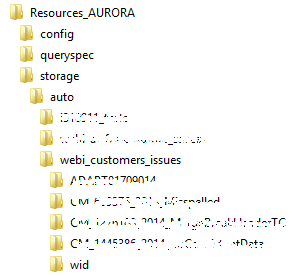
\includegraphics{images/localSavedReferences.png}
  \caption{Capture d'écran de WebI de l'arborescence des références locales}
	\label{figure:localSavedReferences}
\end{figure}
\item[Les logs du serveur tomcat] \hfill \\
Disponible dans le dossier d'installation du serveur ces logs sont trop verbeux pour pouvoir \^{e}tre utiliser, mais sont cependant utiles dans certains cas.
\end{description}





\subsection{De l'\'{e}tude à l'intégration}

Tout d'abord, les requ\^{e}tes de test auto ne sont pas toujours réalisables à notre niveau, il faut donc d'abord vérifier la faisabilité du test. Une fois que l'on a validé que la réalisation est possible et que l'on a choisie une stratégie de test, il faut préparer l'environnement de travail, c'est-à-dire construire la coquille vide du test désiré.


\subsubsection{Analyse du test à implémenter}
\begin{description}
	\item[\'{E}tudier le bug] Au préalable, toutes les informations que l'on a sur le bug a tester se trouvent sur JCWB\index{Java Correction WorkBench}, étudier le workflow provoquant le bug, la description du bug, la/les branche(s) sur laquelle/lesquelles il survient (voir figure \ref{figure:JCWB-CRs} page \pageref{figure:JCWB-CRs})\\
	\begin{figure}[!h]
  \centering
      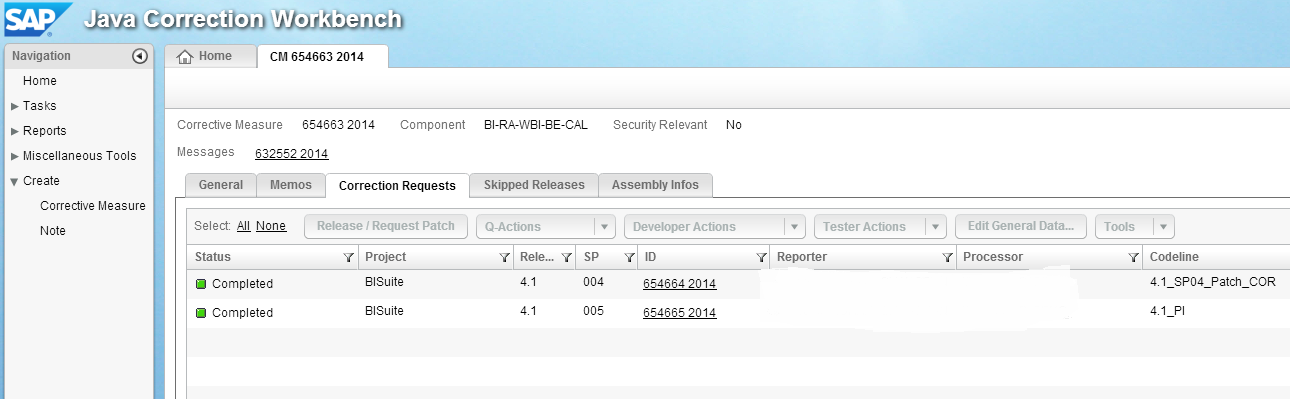
\includegraphics[width=\textwidth]{images/JCWB-CRs.png}
  \caption{\'{E}cran de JCWB propre à une CM\index{Correction Measure}}
	\label{figure:JCWB-CRs}
\end{figure}
Ceci fait, il est intéressant d'aller étudier le code qui a été modifié pour corriger le bug. Pour cela il suffit d'utiliser la fonction \textquote{diff against previous revision} du SCM\index{Source Code Management} pour obtenir la liste exhaustive des fichiers modifiés ainsi qu'un vis-à-vis sur les versions pré-correctif et post-correctif (voir figure \ref{figure:diffAgainst} page \pageref{figure:diffAgainst})\\
	\begin{figure}[!h]
  \centering
      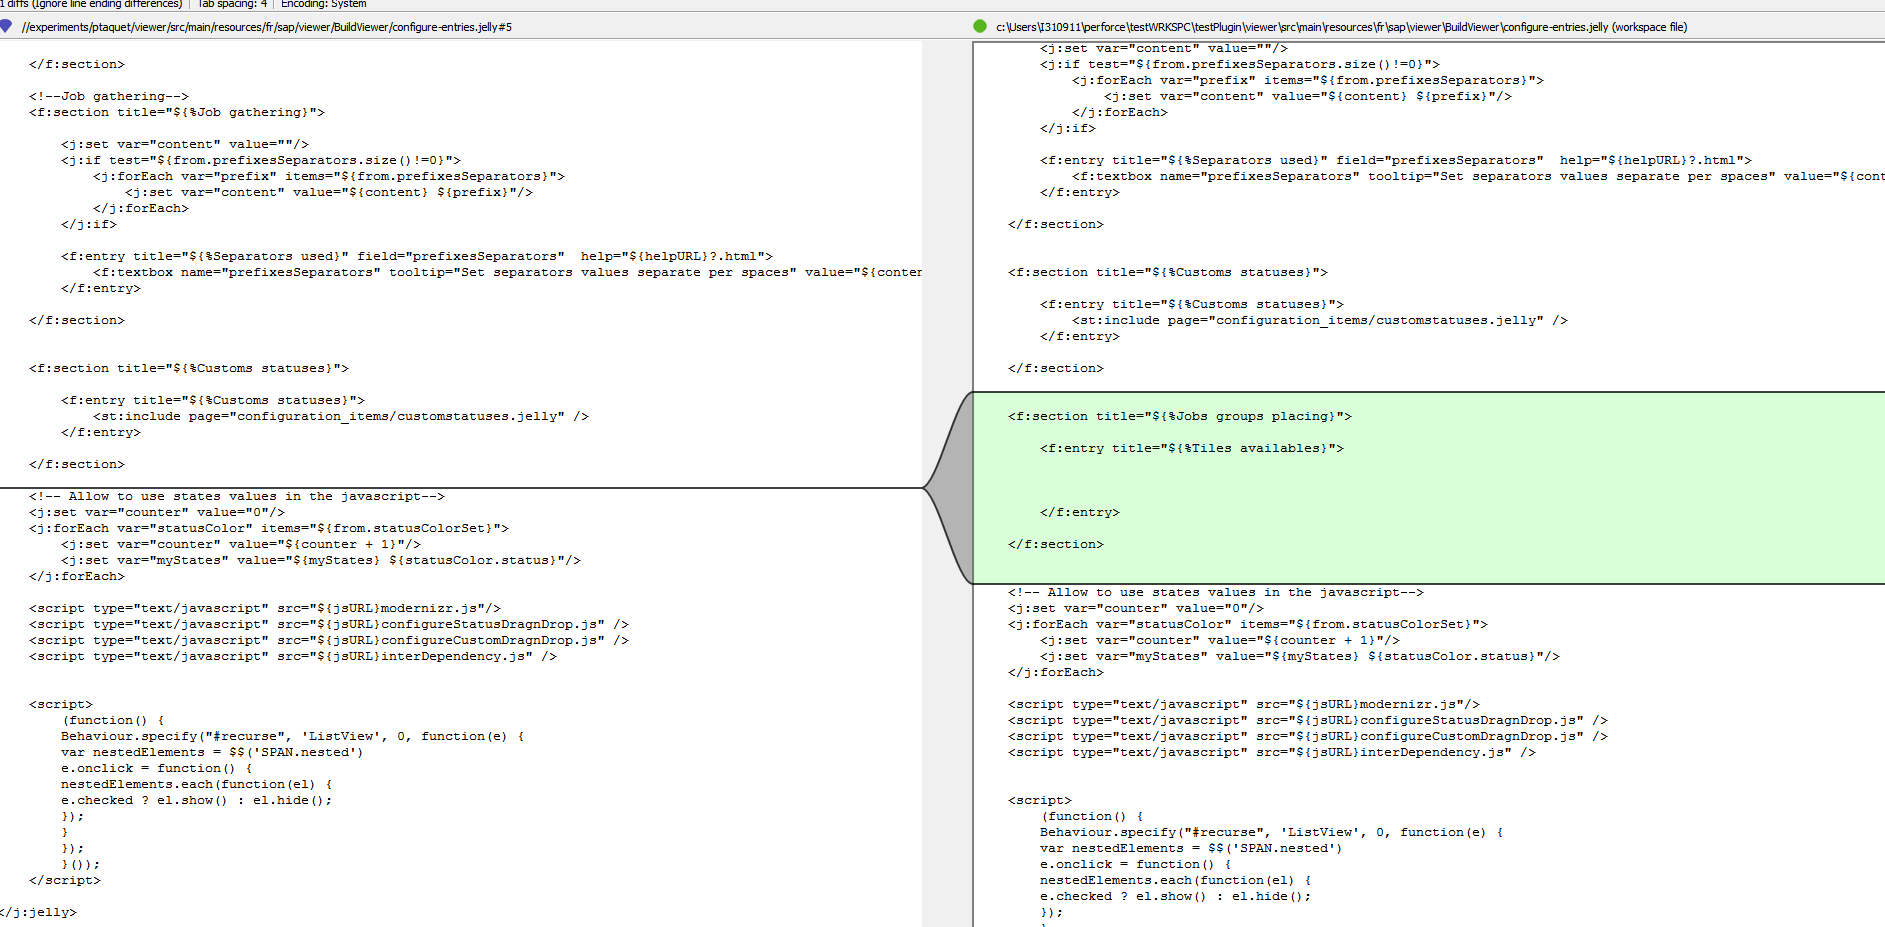
\includegraphics[width=\textwidth]{images/diffAgainst.png}
  \caption{\'{E}cran de comparaison des 2 versions d'un m\^{e}me fichier (avant et après correctif)}
	\label{figure:diffAgainst}
\end{figure}

	\item[Reproduire le problème] Une fois que le bug est bien compris il nous incombe de reproduire à la main le workflow et de valider l'existence du bug sur la version buggée ainsi que le bon fonctionnement de la version corrigée. \`{A} cette étape, si le bug survient sur le CMS\index{CMS} (client léger), il est intéressant d'utiliser le debugger du navigateur pour observer les données transitant.
	
	\item[Définir la stratégie de test] Maintenant que le problème est bien compris et localisé, nous pouvons savoir s'il est possible de le tester. Si non, soit le problème ne peut pas \^{e}tre testé soit nous redirigeons la correction vers l'équipe de testeurs concernée (plus ou moins haut ou bas niveau).\\
Si l'implémentation du test est possible, il faut choisir la meilleure manière de tester l'existence et la non-existence du bug ainsi que le moyen le plus rapide d'arriver à reproduire le problème. Par exemple faut-il un test statique ou dynamique? Partir d'une queryspec\index{queryspec} ou d'un document .wid\index{wid}?
\end{description}


\subsubsection{Implémentation de la coquille vide}
L'intér\^{e}t de coder d'abord la coquille vide est d'avoir un code qui compile mais qui ne fait encore rien. Ce qui garantit que tout se passe correctement au niveau de la nomenclature, la création du test case et, au besoin, la génération sur serveur des .wid\index{wid}.\\ 
Comme sch\'{e}matis\'{e} figure \ref{figure:testsRelations} page \pageref{figure:testsRelations}, chaque test automatique est int\'{e}gr\'{e} \`{a} un test plan, lui-m\^{e}me \'{e}tant int\'{e}gr\'{e}s \`{a} une test suite.\\
\begin{figure}[!h]
  \centering
      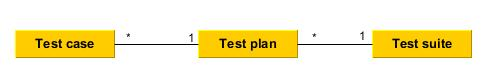
\includegraphics[width=\textwidth]{images/testsRelations.jpg}
  \caption{Diagramme UML des suites de tests}
	\label{figure:testsRelations}
\end{figure}

Ci-dessous les fichiers à implémenter :\\
\begin{enumerate}
	\item \textbf{Test plan} Créer le nouveau test plan dans le package correspondant au client qui a remonté le bug (dans testplan.srebean\_wi.customers.\{clientID\}). Renseigner toutes les informations relatives au test, si ce fichier est correctement implémenté il ne sera plus nécessaire de le modifier par la suite.
	\item \textbf{Test case} Créer le test case dans le package correspondant au client (dans testcases.aurora\_customers.\{clientID\}). Attention à respecter le pattern de nommage \textquote{CM\_\{CM\_id\}\_shortText}.
	\item \textbf{Test suite} Dans le package des tests plan, on peut trouver la test suite qu'il faut modifier. Il suffit de rajouter le nom du test plan à la liste de test plan que la test suite exécute.
	\item \textbf{script.xml} Ajouter les différents paramètres correspondants au test.
	\item \textbf{ressources} Générer les documents ressources nécessaires (queryspec\index{queryspec}, .wid\index{wid}, etc.) et les ajouter au dossier portant le nom de la CM\index{Correction Measure}
	\item \textbf{parameters.xml} Renseigner l'url du CMS\index{CMS} ciblé et mettre à jour les extracted JARs permettant au test vide de compiler
	\item Vérifier l'intégrité de la change list de perforce et finir par push les modification.
\end{enumerate}


D'une manière générale, la structure générale à connaitre pour implémenter correctement la coquille vide est illustrée figure \ref{figure:testEmptyShell} page \pageref{figure:testEmptyShell} 
\begin{figure}[!h]
  \centering
      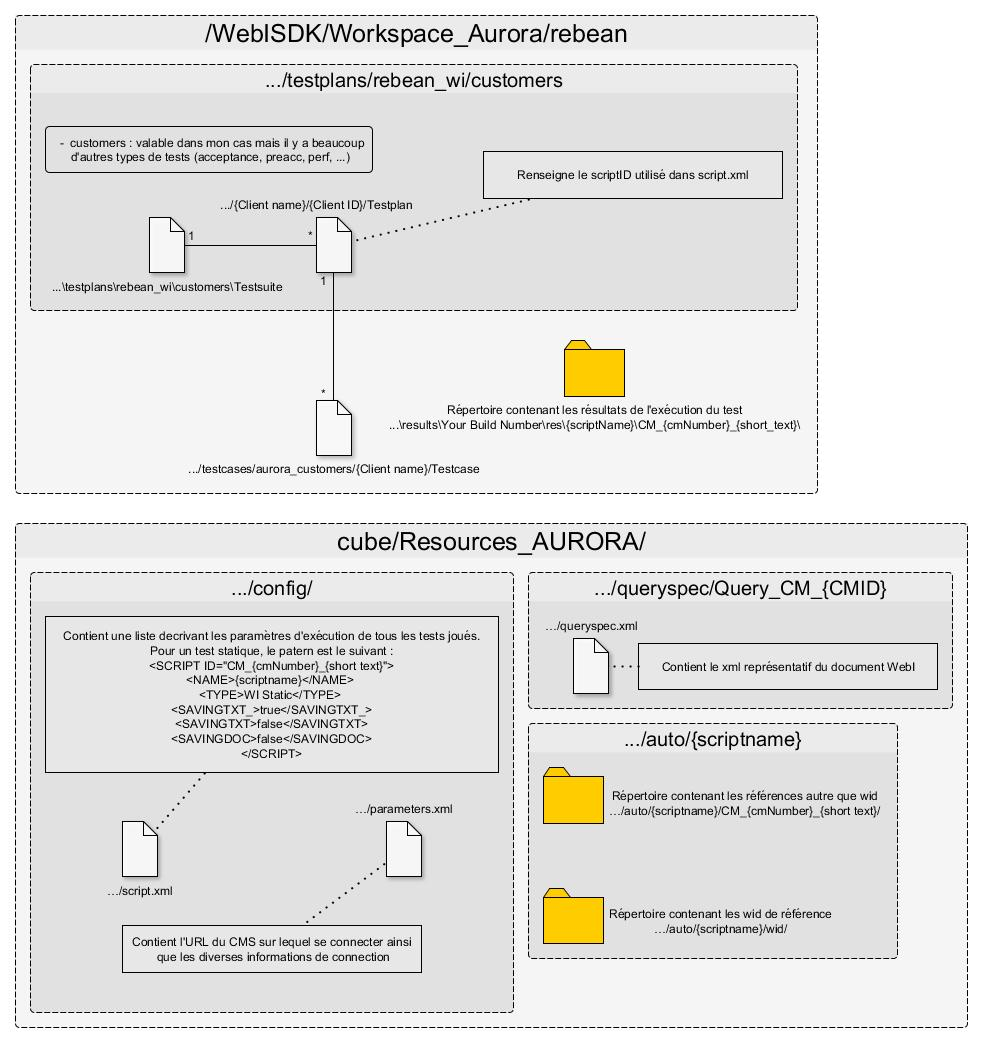
\includegraphics[height=\textheight-1cm]{images/testEmptyShell.jpg}
  \caption{Diagramme représentant les différents éléments qui compose la coquille vide d'un test dynamique}
	\label{figure:testEmptyShell}
\end{figure}

\subsubsection{Les ressources}
Les ressources sont très importantes dans le contexte du test, celles-ci se présentent sous plusieurs jours différents :
\begin{enumerate}
	\item un document .wid\index{wid} créé en suivant à la lettre le workflow à tester mais dont la construction à été arr\^{e}tée juste avant que ne survienne le bug.\\
	Cette ressource sert à utiliser un document déjà construit et permet au ST\index{Software Tester} de n'automatiser que la partie à tester.
	\item un fichier (txt, txt\_, pdf, doc, xls, xls, ...) considéré comme une référence\\
	Cette ressource est comparée au document obtenu à la fin du workflow pour garantir la similitude.
	\item une queryspec\index{queryspec}, c'est un fichier xml représentatif du document .wid\index{wid}
\end{enumerate}

\textbf{Obtenir un fichier wid\index{wid}}
\begin{description}
	\item[Via le CMS\index{CMS}] Il suffit de parcourir l'arborescence du CMS\index{CMS} pour arriver à l'emplacement du .wid\index{wid}. Dans les propiétés du fichier il y a son nom complet (différent du nom dans WebI) avec son arborescence à partir du dossier Input (figure \ref{figure:widFileLocation} page \pageref{figure:widFileLocation} ). Ensuite, dans le système de fichiers du serveur (par exemple : \textquote{\textbackslash{}\textbackslash{}dewdftv01634.dhcp.pgdev.sap.corp\textbackslash{}c\$}) aller dans 
	\textquote{\textbackslash{}Program Files (x86)\textbackslash{}SAP BusinessObjects\textbackslash{}SAP BusinessObjects Enterprise XI 4.0\textbackslash{}FileStore\textbackslash{}Input} et copier/coller le chemin d'accès au fichier. Le document .wid\index{wid} se trouve dans le répertoire en question.
	\begin{figure}[!h]
  \centering
      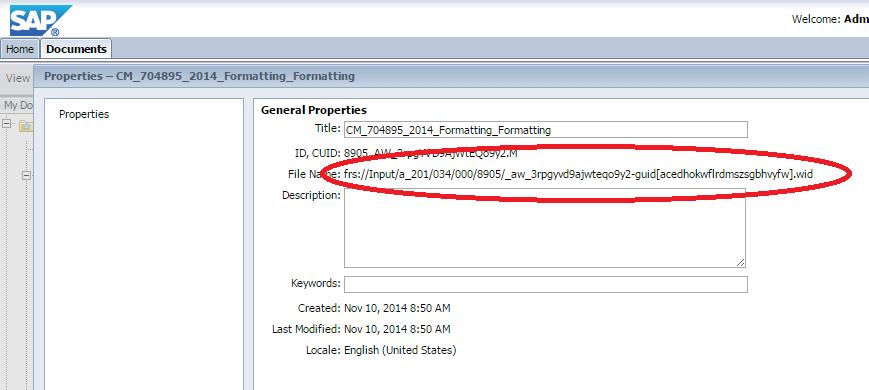
\includegraphics[width=\textwidth]{images/widFileLocation.png}
  \caption{Capture de l'écran de propriété d'un document WebI}
	\label{figure:widFileLocation}
\end{figure}
	\item[Via le Rich Client]
	Attention à la version du rich client qui doit \^{e}tre la m\^{e}me que celle du CMS\index{CMS}. Ouvrir une connexion pointée sur le bon CMS\index{CMS}, ouvrir le document désiré et enregistrer sous le document .wid\index{wid}.
\end{description}

\section{Bilan de mes 1\up{\`{e}res} missions}
Tout au long des mois de juillet, ao\^{u}t et septembre j'ai implémenter beaucoup de tests\footnote{cf. annexe \ref{pdf:ImplementedTestsList} page \pageref{pdf:ImplementedTestsList} pour la liste compl\`{e}te des tests impl\'{e}ment\'{e}s} pour des bugs divers et à l'impact plus ou moins critique. J'ai beaucoup appris de mes erreurs, surtout lorsque plusieurs jours de travail s'avéraient inutiles parce qu'une meilleure solution, évidente pour qui sait, existait.


\subsection{Les 1\up{\`{e}res} erreurs}

Les principales pertes de temps : coder des choses inutiles ou d\'{e}j\`{a} existantes.\\
r\'{e}inventer la roue. Beaucoup de choses que j'ai cod\'{e} se sont av\'{e}r\'{e}s \^{e}tre d\'{e}j\`{a} existantes dans le framework

perdre du temps \`{a} impl\'{e}menter des choses inutiles (exemple : cr\'{e}ation d'un doc niv sdk\index{SDK} alors que l'on peut juste  le r\'{e}cup\'{e}rer)

Casser la build : ne jamais push le vendredi soir au risque de casser la build du week-end.

\subsection{Les acquis}
ce qu'il faut faire pour tester

comprendre le test (\'{e}tudier le workflow et cibler exactement la partie du workflow \`{a} tester)
mettre en place la coquille vide du test et g\'{e}n\'{e}rer et/ou r\'{e}cup\'{e}rer les fichiers utiles au d\'{e}veloppement et/ou \`{a} l'ex\'{e}cution du test.
Tester le test! ie ex\'{e}cuter sur 2 versions, l'une fix\'{e}e l'autre non.
push le test\\ 

ne jamais push le vendredi soir

la composition d'un document WebI au niveau SDK\index{SDK}

